\documentclass[aspectratio=169,11pt]{beamer}

\usepackage{amsmath,amssymb,bm}
\usepackage{mathtools}
\usepackage{booktabs}
\usepackage{graphicx}
\usepackage{tikz}

\usetheme{metropolis}
\setbeamertemplate{navigation symbols}{}

% Fallback if metropolis isn't available locally:
\IfFileExists{beamerthememetropolis.sty}{}{%
  \usetheme{default}%
  \usecolortheme{seahorse}%
  \setbeamertemplate{frametitle}[default][center]%
}

\newcommand{\Hop}{\hat{H}}
\newcommand{\Vop}{\hat{V}}
\newcommand{\Eint}{\Delta E_{\mathrm{int}}}
\newcommand{\Eiso}{E^{(\mathrm{iso})}}
\newcommand{\Ecpl}{E_{\mathrm{complex}}}

\title{Energy decomposition of molecular complexes}
\subtitle{From the Schr\"odinger equation to a many-body expansion on \textsc{MACE}}
\author{}
\date{}

\begin{document}

\maketitle

% ---------------------------------------------------------------- %
\begin{frame}{Setting}
A complex of $M$ molecules
$\mathcal{C}=\{1,\dots,M\}$, nuclei partitioned by molecule
$\{A\}=\bigsqcup_{\alpha=1}^{M}\mathcal{N}_\alpha$.

\bigskip
For any non-empty $S\subseteq\mathcal{C}$, write $E(S)$ for the
exact ground-state electronic energy of the isolated sub-system that
contains the molecules indexed by $S$.

\bigskip
Shorthand:
\[
\Ecpl \equiv E(\mathcal{C}),
\qquad
\Eiso_\alpha \equiv E(\{\alpha\}).
\]

\bigskip
\textbf{Question.} \;Can we cleanly split
$\Ecpl$ into self-energies of the molecules and interaction energies?
\end{frame}

% ---------------------------------------------------------------- %
\begin{frame}{Hamiltonian: an operator-level split}
Born--Oppenheimer electronic Hamiltonian, in atomic units:
\[
\Hop = -\tfrac12\!\sum_{i}\nabla_i^2
\;-\;\sum_{i,A}\!\frac{Z_A}{|\mathbf r_i-\mathbf R_A|}
\;+\;\sum_{i<j}\!\frac{1}{|\mathbf r_i-\mathbf r_j|}
\;+\;\sum_{A<B}\!\frac{Z_A Z_B}{|\mathbf R_A-\mathbf R_B|}.
\]

Splitting every two-index sum into ``same-molecule'' and
``cross-molecule'' parts gives
\[
\boxed{\;\Hop \;=\; \sum_{\alpha=1}^{M}\Hop_\alpha^{(0)}
       \;+\;\Vop_{\mathrm{int}}.\;}
\]
\begin{itemize}\setlength\itemsep{2pt}
\item $\Hop_\alpha^{(0)}$: the Hamiltonian one would write down for an
\emph{isolated} molecule $\alpha$.
\item $\Vop_{\mathrm{int}}$: every term whose two indices belong to
different molecules.
\end{itemize}

\textbf{So far so clean.}\;
But operator additivity does not yet imply energy additivity.
\end{frame}

% ---------------------------------------------------------------- %
\begin{frame}{Two obstacles to a per-molecule decomposition}
\small
\textbf{(i) Indistinguishability of electrons.}\;
The exact ground state $\Psi$ must be antisymmetric under exchange of
\emph{any} two electrons --- including across molecules. There is no
QM observable that ``labels'' an electron as molecule-$\alpha$'s, so
\[
\langle\Psi|\Hop_\alpha^{(0)}|\Psi\rangle \;\neq\; \Eiso_\alpha
\qquad \text{in general.}
\]

\medskip
\textbf{(ii) Non-uniqueness of a finer decomposition.}\;
What \emph{is} unambiguous is the supersystem difference
\[
\boxed{\;\Eint \;\equiv\; \Ecpl \;-\; \sum_{\alpha=1}^{M}\Eiso_\alpha\;}
\]
(rigorous; basis-set-dependent in finite basis $\to$ counterpoise / BSSE).
Splitting $\Eint$ further into electrostatic / exchange / dispersion /
charge-transfer is scheme-dependent (SAPT, EDA, ALMO-EDA, \dots);
different schemes give different numbers.
\end{frame}

% ---------------------------------------------------------------- %
\begin{frame}{The many-body expansion --- recursive definition}
For non-empty $S\subseteq\mathcal{C}$, define $n$-body energies
recursively on $|S|$:
\begin{align*}
\Delta E^{(1)}_{\{\alpha\}}            \;&=\; \Eiso_\alpha,\\[1pt]
\Delta E^{(2)}_{\{\alpha,\beta\}}      \;&=\; E(\{\alpha,\beta\})-\Eiso_\alpha-\Eiso_\beta,\\[1pt]
\Delta E^{(3)}_{\{\alpha,\beta,\gamma\}}\;&=\; E(\{\alpha,\beta,\gamma\})
   -\!\!\!\sum_{\delta\in\{\alpha,\beta,\gamma\}}\!\!\Eiso_\delta
   -\!\!\!\!\sum_{\substack{T\subset\{\alpha,\beta,\gamma\}\\|T|=2}}\!\!\!\!\Delta E^{(2)}_T,
\end{align*}
and in general
\[
\boxed{\;
\Delta E^{(n)}_{S}
\;\equiv\; E(S)\;-\!\!\sum_{\varnothing\ne T\subsetneq S}\!\!\Delta E^{(|T|)}_{T}.\;}
\]

\smallskip
Interpretation: $\Delta E^{(n)}_S$ is the part of $E(S)$ that no
proper-subset cluster can capture --- the irreducible $n$-body
correction.
\end{frame}

% ---------------------------------------------------------------- %
\begin{frame}{M\"obius inversion: closed form}
Solving the recursion gives the explicit closed form
\[
\boxed{\;
\Delta E^{(n)}_{S}
\;=\;\sum_{T\subseteq S}(-1)^{|S|-|T|}\,E(T),\qquad |S|=n.\;}
\]
Equivalently,
\[
E(S)\;=\;\sum_{\varnothing\ne T\subseteq S}\Delta E^{(|T|)}_T.
\]

\medskip
\textbf{Properties.}
\begin{itemize}\setlength\itemsep{2pt}
\item Permutation-symmetric in the labels of $S$.
\item Sign pattern: alternating with $|S|-|T|$ (inclusion--exclusion).
\item Truncating at order $n^\star$ requires
$\sum_{n=1}^{n^\star}\binom{M}{n}$ sub-system calculations.
\item Convergence is fast for short-ranged, weakly polarising
interactions; slow for metallic / strongly delocalised systems.
\end{itemize}
\end{frame}

% ---------------------------------------------------------------- %
\begin{frame}{Total-energy expansion}
\small
Specialise $S=\mathcal{C}$:
\[
\boxed{\;
\Ecpl
\;=\;\sum_{\alpha}\Eiso_\alpha
\;+\;\sum_{\alpha<\beta}\Delta E^{(2)}_{\{\alpha,\beta\}}
\;+\;\sum_{\alpha<\beta<\gamma}\Delta E^{(3)}_{\{\alpha,\beta,\gamma\}}
\;+\;\cdots
\;+\;\Delta E^{(M)}_{\mathcal{C}}.\;}
\]
Equivalently, the rigorous interaction energy is
\[
\Eint \;=\; \Ecpl - \sum_\alpha\Eiso_\alpha
\;=\;\sum_{n=2}^{M}\,\sum_{\substack{S\subseteq\mathcal{C}\\|S|=n}}\Delta E^{(n)}_{S}.
\]

\textbf{Bottom line.}
\begin{itemize}\setlength\itemsep{1pt}
\item The two-way split (self $+$ interaction) is clean and unique.
\item The $n$-body refinement is unique once the convention above is fixed.
\item Component decomposition (electrostatic / exchange / dispersion
/$\,\dots$) is \emph{not} unique --- it depends on the chosen scheme.
\end{itemize}
\end{frame}

% ---------------------------------------------------------------- %
\begin{frame}{Worked example: $M=4$}
For $\mathcal{C}=\{1,2,3,4\}$ the Möbius form spells out:
{\small
\begin{align*}
\Delta E^{(2)}_{\{1,2\}} &= E(\{1,2\}) - \Eiso_1 - \Eiso_2,\\[2pt]
\Delta E^{(3)}_{\{1,2,3\}} &= E(\{1,2,3\})
  -\!\!\sum_{\alpha\in\{1,2,3\}}\!\!\Eiso_\alpha
  -\!\!\!\!\sum_{\substack{T\subset\{1,2,3\}\\|T|=2}}\!\!\!\!\Delta E^{(2)}_T,\\[2pt]
\Delta E^{(4)}_{\{1,2,3,4\}}
 &=\;E(\{1,2,3,4\})\\
 &\;-\;\big[E(\{1,2,3\})+E(\{1,2,4\})+E(\{1,3,4\})+E(\{2,3,4\})\big]\\
 &\;+\;\big[E(\{1,2\})+E(\{1,3\})+E(\{1,4\})+E(\{2,3\})+E(\{2,4\})+E(\{3,4\})\big]\\
 &\;-\;\big[\Eiso_1+\Eiso_2+\Eiso_3+\Eiso_4\big].
\end{align*}}%
Pattern: $\binom{4}{n}$ terms of size $n$, alternating signs.
\end{frame}

% ================================================================ %
% Effective surfaces from a focus set
% ================================================================ %
\begin{frame}{Effective surfaces: motivation}
\small
Exploring the conformational landscape we don't always want
\emph{every} minimum of $\Ecpl$. A common case: some fragments are the actors
of interest, the rest are bystanders, and configurations in which two
bystanders cluster with each other far from the actors are deep but
irrelevant minima.

\medskip
\textbf{Idea.}\,Pick a \emph{focus set} $F\subseteq\mathcal{C}$. From the MBE,
keep every term whose subset $S$ intersects $F$, and discard every term
confined to spectators:
\[
E_{\mathrm{eff}}^{F}
\;\equiv\!\!\!\!\sum_{\substack{S\subseteq\mathcal{C}\\ S\cap F\ne\varnothing}}
\!\!\!\!\Delta E^{(|S|)}_S.
\]
Every spectator-only cluster ($S\cap F=\varnothing$) is cancelled exactly.

\medskip
The resulting surface is flat in directions that move bystanders around among
themselves while keeping them outside the receptive field of $F$ — the
spurious minima vanish by construction.
\end{frame}

% ---------------------------------------------------------------- %
\begin{frame}{Effective surfaces: closed form}
\small
The same identity $E(S)=\sum_{T\subseteq S}\Delta E^{(|T|)}_T$, applied once
to $\mathcal{C}$ and once to $\mathcal{C}\setminus F$ and subtracted,
collapses the sum:
\[
\boxed{\;E_{\mathrm{eff}}^{F}
\;=\;E(\mathcal{C})\;-\;E(\mathcal{C}\setminus F).\;}
\]
To make the surface vanish when $F$ is removed to infinity from spectators,
subtract the focus-only energy:
\[
E_{\mathrm{eff}}^{F,\,0}
\;=\;E(\mathcal{C})\;-\;E(\mathcal{C}\setminus F)\;-\;E(F).
\]

\textbf{Cost.}\,Two (or three) energy evaluations \emph{regardless} of $M$;
no $\binom{M}{n}$ enumeration. Trivial driver around the forward pass.

\textbf{Properties.}\,Spectator-gauge invariance (spectator-only minima are
flat); cooperativity preserved (three- and higher-body terms involving $F$
remain at every order); spectator self-forces cancel atom-by-atom under
$\nabla_{\mathbf r}$, leaving only $F$-mediated forces.
\end{frame}

% ---------------------------------------------------------------- %
\begin{frame}{Worked example: 4 NH$_3$ + Cu$^{+}$, focus $F=\{$Cu$\}$}
\footnotesize
Take $F=\{\text{Cu}\}$. Then \emph{every} term in $E_{\mathrm{eff}}^F$
involves Cu; every term confined to NH$_3$ fragments is cancelled.

\medskip
\centering
\renewcommand{\arraystretch}{1.05}
\begin{tabular}{l@{\;}c@{\;}c@{\;}c}
\toprule
MBE term type & Total & Kept & Dropped \\
\midrule
$\Delta E^{(1)}$  ($\Eiso_\alpha$)   & 5  & 1 (Cu)              & 4 (each NH$_3$) \\
$\Delta E^{(2)}$  (pairs)            & 10 & 4 (Cu--NH$_3$)      & 6 (NH$_3$--NH$_3$) \\
$\Delta E^{(3)}$  (triples)          & 10 & 6 (Cu--NH$_3$--NH$_3$) & 4 (NH$_3^{\times 3}$) \\
$\Delta E^{(4)}$  (quadruples)       & 5  & 4 (Cu + 3 NH$_3$)    & 1 (NH$_3^{\times 4}$) \\
$\Delta E^{(5)}$  (full)             & 1  & 1                    & 0 \\
\midrule
Total                                & 31 & \textbf{16}          & \textbf{15} \\
\bottomrule
\end{tabular}

\medskip
\flushleft
\textbf{Implementation: three forward passes.}
\[
E_{\mathrm{eff}}^{\{\text{Cu}\},\,0}
\;=\;\underbrace{E(\text{4 NH}_3+\text{Cu})}_{\text{full complex}}
\;-\;\underbrace{E(\text{4 NH}_3\text{ at same positions})}_{\text{spectators only, charge 0}}
\;-\;\underbrace{E(\text{Cu}^+)}_{\text{focus baseline}}.
\]
\end{frame}

% ---------------------------------------------------------------- %
\begin{frame}{Numerical experiment}
\textbf{System:} $4\,\mathrm{NH}_3 + \mathrm{Cu}^{+}$ \;($M=5$, $17$ atoms).

\textbf{Sampler:} \texttt{PolyChem-sisnf} spherical-coordinate prior
($r_{\max}=5\,$\AA), random parameter vector
$x\sim\mathcal{U}([0,1]^{21})$.

\textbf{Energy model:} \textsc{MACE-jax} \texttt{mace-omol-0}
(neutral DFT-trained; $r_{\max}=6\,$\AA, $L=3$ message-passing layers;
charge \& spin embeddings).

\textbf{Procedure.} For each random geometry, compute
$E(S)$ for all $2^{M}-1=31$ non-empty subsets $S$ of fragments;
apply the M\"obius identity to get every $\Delta E^{(n)}_S$.

\bigskip
\textbf{Sanity check.}\;\;The MBE telescopes exactly:
$\displaystyle \sum_{S}\Delta E^{(|S|)}_S \;=\; \Ecpl$ to machine precision
(observed residual $0.00\times 10^{0}$ eV in single precision).
\end{frame}

% ---------------------------------------------------------------- %
\begin{frame}{How to read the next slides}
\small
Each upcoming geometry slide shows the structure on the left and its
full MBE on the right.

\medskip
\textbf{Left panel.} 3D structure, atoms coloured by fragment.

\medskip
\textbf{Right, top.} Five 1-body terms
$\Delta E^{(1)}_{\{\alpha\}}=\Eiso_\alpha$ on a symmetric-log axis
(NH$_3$: $\sim\!-1.5\times10^{3}$ eV;\;Cu$^{+}$: $\sim\!-4.5\times10^{4}$ eV).

\medskip
\textbf{Right, bottom.} All 26 interaction terms $\Delta E^{(n)}_S$
with $n\ge2$:
\(\binom{5}{2}{=}10\) pairs,\;
\(\binom{5}{3}{=}10\) triples,\;
\(\binom{5}{4}{=}5\) quadruples,\;
\(1\) five-body term.

\medskip
The slide title reports
$\sum_S \Delta E^{(|S|)}_S = \Ecpl$ --- the M\"obius identity holds
exactly.

\bigskip
\textbf{Order:}\;
(1) symmetric tetrahedral optimum,\;
(2) two close + two far,\;
(3) four random geometries from the prior.
\end{frame}

% ================================================================ %
% (1) Tetrahedral
% ================================================================ %
\begin{frame}{(1) Symmetric tetrahedral [Cu(NH$_3$)$_4$]$^{+}$}
\begin{columns}[T]
\begin{column}{0.55\textwidth}
\textbf{Construction.}
\begin{itemize}\setlength\itemsep{1pt}
\item Cu at the origin.
\item Four NH$_3$ at the vertices of a regular tetrahedron;
each $C_{3v}$ axis radial outward (lone pair pointing at Cu, H tripod
on the far side).
\item Internal NH$_3$ from the PolyChem-sisnf zmat:
$d_{\mathrm{NH}}=1.0127\,$\AA,\;\; $\angle\mathrm{HNH}=107.6432^{\circ}$.
\end{itemize}

\medskip
\textbf{1D grid search.}
\begin{itemize}\setlength\itemsep{1pt}
\item Coarse grid $1.6$--$3.5\,$\AA\ (20 points).
\item Fine grid centred on the coarse minimum (41 points).
\item Symmetry $\to$ one Cu--N distance parametrises the whole complex.
\end{itemize}

\medskip
\textbf{Result.}
\(d^{*}_{\mathrm{Cu-N}}=2.175\,\)\AA,\;
\(E^{*}=-50791.34\,\)eV.
Lower than every random sample by $5$--$9$ eV.
\end{column}
\begin{column}{0.45\textwidth}
\centering
\includegraphics[width=\linewidth]{mbe_figures/geom_tet_scan.png}
\end{column}
\end{columns}
\end{frame}

\begin{frame}[plain]
\begin{center}
\includegraphics[width=\paperwidth,height=\paperheight,keepaspectratio]
  {mbe_figures/geom_tet.png}
\end{center}
\end{frame}

% ================================================================ %
% (2) Two close + two far
% ================================================================ %
\begin{frame}{(2) Two close + two far}
\small
\begin{columns}[T]
\begin{column}{0.58\textwidth}
\textbf{Construction.}
\begin{itemize}\setlength\itemsep{1pt}
\item Cu at origin; NH$_3$\#1c, NH$_3$\#2c at $\pm z$ with
$d_{\mathrm{Cu-N}}=2.175\,$\AA, $C_{3v}$ axes radial outward.
\item NH$_3$\#3f, NH$_3$\#4f at $(9,\pm1.7,0)\,$\AA\ as an H-bonded
dimer (donor rotated so one H sits on the dimer axis, H$\cdots$N
$=2.39\,$\AA).
\end{itemize}

\medskip
\textbf{Physical expectation.} Strong Cu--NH$_3$\#1c, Cu--NH$_3$\#2c
pair terms $\approx -1.4\,$eV each; weak H-bond
$\approx -0.13\,$eV; all Cu$\leftrightarrow$far cross terms $\approx 0$
(beyond $r_{\max}$).
\end{column}
\begin{column}{0.42\textwidth}
\vspace*{4mm}
\centering
\textit{Construction sketch:}\\[2pt]
\scalebox{0.78}{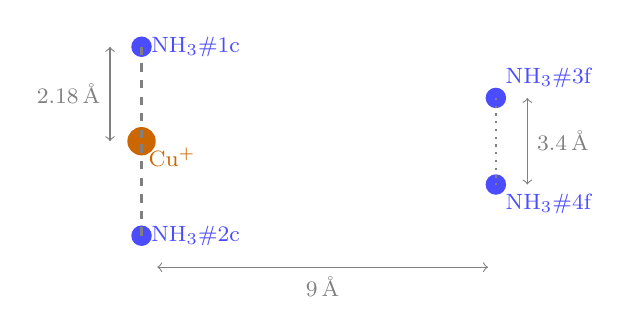
\begin{tikzpicture}[font=\footnotesize]
\fill[orange!80!black] (0,0) circle (0.18) node[below right=-1pt] {Cu$^{+}$};
\fill[blue!70] (0,1.2) circle (0.13) node[right] {NH$_3$\#1c};
\fill[blue!70] (0,-1.2) circle (0.13) node[right] {NH$_3$\#2c};
\fill[blue!70] (4.5, 0.55) circle (0.13) node[above right] {NH$_3$\#3f};
\fill[blue!70] (4.5,-0.55) circle (0.13) node[below right] {NH$_3$\#4f};
\draw[dashed,thick,gray] (0,1.2) -- (0,0); \draw[dashed,thick,gray] (0,-1.2) -- (0,0);
\draw[dotted,thick,gray] (4.5,0.55) -- (4.5,-0.55);
\draw[<->,gray] (-0.4,0) -- (-0.4,1.2) node[midway,left]{2.18\,\AA};
\draw[<->,gray] (4.9,0.55) -- (4.9,-0.55) node[midway,right]{3.4\,\AA};
\draw[<->,gray] (0.2,-1.6) -- (4.4,-1.6) node[midway,below]{9\,\AA};
\end{tikzpicture}}
\end{column}
\end{columns}

\medskip
\textbf{Caveat: charge-embedding artefact.}\;
The figure on the next slide will show
$\Delta E^{(3)}_{\{\mathrm{NH_3\#3f},\mathrm{NH_3\#4f},\mathrm{Cu}\}}\sim+8\,$eV.
This is \emph{not} a physical 3-body interaction; the OMol model's
$+1$ total charge is global, so when Cu shares a graph with the far
dimer the model spreads charge across the dimer and shifts its energy.
The MBE dumps the discrepancy into a high-order term.
\end{frame}

\begin{frame}[plain]
\begin{center}
\includegraphics[width=\paperwidth,height=\paperheight,keepaspectratio]
  {mbe_figures/geom_2c2f.png}
\end{center}
\end{frame}

% ================================================================ %
% (3) Random samples from the prior
% ================================================================ %
\begin{frame}{(3) Random samples from the spherical-coordinate prior}
For comparison, four geometries drawn uniformly from
$x\sim\mathcal{U}([0,1]^{21})$ via the same prior used by the nested
sampler. Each is shown with its full MBE.

\medskip
\textbf{Expectation.} Since the prior does not enforce
\texttt{min\_atom\_distance} or any chemical bias, some geometries
will place NH$_3$ molecules unphysically close to Cu (clash
penalty $\to$ positive 2-body) or far from any partner (interactions
$\to 0$). Geometries that happen to be near tetrahedral coordination
should approach the optimum from slide~(1).
\end{frame}

\begin{frame}[plain]
\begin{center}
\includegraphics[width=\paperwidth,height=\paperheight,keepaspectratio]
  {mbe_figures/geom_00.png}
\end{center}
\end{frame}

\begin{frame}[plain]
\begin{center}
\includegraphics[width=\paperwidth,height=\paperheight,keepaspectratio]
  {mbe_figures/geom_01.png}
\end{center}
\end{frame}

\begin{frame}[plain]
\begin{center}
\includegraphics[width=\paperwidth,height=\paperheight,keepaspectratio]
  {mbe_figures/geom_02.png}
\end{center}
\end{frame}

\begin{frame}[plain]
\begin{center}
\includegraphics[width=\paperwidth,height=\paperheight,keepaspectratio]
  {mbe_figures/geom_03.png}
\end{center}
\end{frame}

% ================================================================ %
% Effective-surface annotation on the same figures
% ================================================================ %
\begin{frame}{Re-reading the previous figures with $F=\{$Cu$\}$}
\small
Same MBE numerics as before, but now MBE bars are coloured by whether
they survive in $E_{\mathrm{eff}}^F$:
\begin{itemize}\setlength\itemsep{1pt}
\item \textbf{Coloured bars.}\;Subset $S$ contains Cu; the term is kept ---
contributes to $E_{\mathrm{eff}}^F$.
\item \textbf{Grey bars.}\;Subset $S$ is confined to NH$_3$ fragments;
the term is cancelled in $E(\mathcal{C})-E(\mathcal{C}\setminus F)$ ---
\emph{not} part of the effective surface.
\end{itemize}
The figure suptitle reports the surviving sum
$E_{\mathrm{eff}}^F = \sum_{S\cap F\neq\varnothing}\Delta E^{(|S|)}_S$ and
the dropped spectator-only sum.

\medskip
\textbf{What to look for.}
\begin{itemize}\setlength\itemsep{1pt}
\item \textbf{Tetrahedral.}\;The dropped block is essentially $4\Eiso_{\rm NH_3}$
plus tiny inter-NH$_3$ pair terms. The kept block carries all of the
chemically meaningful Cu coordination.
\item \textbf{Two close + two far.}\;The grey NH$_3$\#3f--NH$_3$\#4f H-bond
($-0.13$ eV) is dropped --- the spurious "spectator dimer" minimum is
gone from $E_{\mathrm{eff}}^F$. The yellow 5-body bar (which carries the
charge-embedding artefact) is \emph{kept}, since it contains Cu.
\end{itemize}
\end{frame}

\begin{frame}[plain]
\begin{center}
\includegraphics[width=\paperwidth,height=\paperheight,keepaspectratio]
  {mbe_figures/geom_tet_focus.png}
\end{center}
\end{frame}

\begin{frame}[plain]
\begin{center}
\includegraphics[width=\paperwidth,height=\paperheight,keepaspectratio]
  {mbe_figures/geom_2c2f_focus.png}
\end{center}
\end{frame}

\end{document}
